%
% Created       : 2014 Jul 21 (Mon) 10:47:41 by Harold Carr.
% Last Modified : 2015 May 08 (Fri) 18:05:00 by Harold Carr.
%

% \documentclass[convert={density=300,size=1080x800,outext=.png}]{standalone}
% \documentclass[convert={density=300,outext=.png}]{standalone}
\documentclass[convert={density=175,outext=.png}]{standalone}

\usepackage{tikz}
\usetikzlibrary{matrix,arrows}

\begin{document}

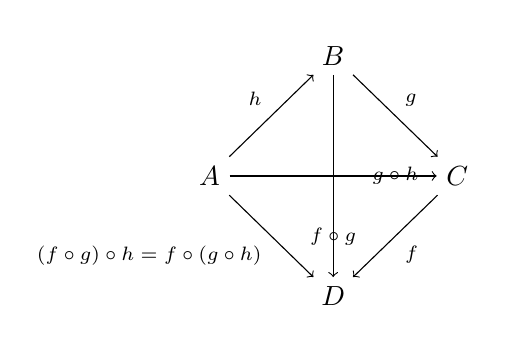
\begin{tikzpicture}[descr/.style={fill=white,inner sep=2.5pt}]
\matrix (m) [matrix of math nodes, row sep=3em, column sep=3em]
{   & B &  \\
  A &   & C \\
    & D &   \\
};
\path[->,font=\scriptsize]
(m-2-1) edge node[auto]      {$ h           $}                               (m-1-2)
(m-1-2) edge node[auto]      {$ g           $}                               (m-2-3)
(m-2-1) edge node[pos=0.8]   {$ g \circ h $}                                 (m-2-3)
(m-2-1) edge node[auto,swap] {$ (f \circ g) \circ h = f \circ (g \circ h) $} (m-3-2)
(m-2-3) edge node[auto]      {$ f         $}                                 (m-3-2)
(m-1-2) edge node[pos=0.8]   {$ f \circ g $}                                 (m-3-2)
;
\end{tikzpicture}

\end{document}

% End of file.
